\section{Blokų grandine paremtas tapatybės atributų valdymo modelis} \label{section:BCIDM}

Atsižvelgus į blokų grandinės savybes, tinkamas tapatybės valdymo problemoms spręsti, šiame skyriuje pateikiamas
blokų grandine paremtas skaitmeninės tapatybės valdymo modelis. Modelis skirtas spręsti\hypertarget{IDM:problemsSummarized}{~\ref{IDM:problemsSummarized}} skyrelyje
apibendrintoms naudotojų problemoms. Kadangi tapatybės valdymas apima
daug skirtingų procesų, aprašomas modelis apsiriboja asmens tapatybės atributų valdymu ir perdavimu. Kuriamo modelio architektūra 
remiasi MIT tyrime \cite{MITPaper} pristatytais teoriniais protokolais, bandant juos modifikuoti ir pritaikyti
ne tik mobiliosioms aplikacijoms, o ir interneto tinklalapiams.

\subsection{Reikalavimai} \label{BCIDM:requirements}

Naudotojams kylančios problemos tapatybės valdyme remiasi į tai, kad jų tapatybė yra
visiškai patikėta valdyti tapatybės tiekėjams. Dėl menko naudotojų įsitraukimo į tapatybės valdymo
procesus, asmenys neretai lieka tik pasyvūs stebėtojai.

Siekiant išspręsti šią problemą, kuriamo modelio reikalavimai kurti pagal į naudotoją orientuotos tapatybės
(angl. \textit{user-centric identity}) principus. Ši paradigma akcentuoja naudotojus kaip centrinę
identiteto valdymo sistemų dalį, perduodant paslaugų ir tapatybės tiekėjų turimą tapatybės kontrolę
naudotojams \cite{Cao2010}. Tokiu būdu, naudotojai turi aktyviau prižiūrėti ir dalyvauti tapatybės
valdymo procesuose (dažniausiai naudojant papildomą programinę įrangą),
tačiau geriau žino, kaip ir kur yra naudojami jų asmens duomenys.

Taikant į asmenis orientuotos skaitmeninės tapatybės principus, reikalavimai modeliui suformuluoti naudotojų istorijų forma:

\begin{enumerate}
    \item Kaip interneto naudotojas, aš noriu žinoti, kurios programos turi prieigą prie kurių mano asmens duomenų.
    \item Kaip interneto naudotojas, aš noriu kontroliuoti savo asmens duomenis ir pats suteikti arba atmesti prieigą paslaugų tiekėjams pasiekti mano duomenis.
    \item Kaip interneto naudotojas, aš noriu galimybės lengvai atnaujinti savo asmens duomenis vienoje vietoje.
    \item Kaip interneto naudotojas, aš nenoriu, jog mano asmens duomenų pasiekiamumas priklausytų tik nuo vienos trečiosios šalies pasiekiamumo.
\end{enumerate}

Pateiktos naudotojų istorijos padengia 1 skyriuje apibrėžtus asmenų poreikius tapatybės valdymo
sistemoms bei išskirtas kontrolės, pasitikėjimo ir skaidrumo trūkumo problemas. Interneto tapatybių valdymo sistemo saugumo atakos (angl.
\textit{cross site scripting}, \textit{phishing}) yra plati tema, verta atskiro tyrimo, tad ji šiame modelyje nebus nagrinėjama. \textcolor{red}{ar užtenka tokio sakinio pasakymui kad čia \textit{out of scope}? nes saugumui užtikrint reik
kad naudojamos paslaugos SSL turėtų, ir šiaip plati tema labai, kurios vien blockchain neišspręs}

\subsection{Modelio dalys}

Modelis sudarytas iš trijų dalių: išmaniųjų kontraktų paslaugų autorizavimo logikai bei atributų saugojimui,
atributų valdymo programos bei paslaugų registro.

\subsubsection{Išmanieji kontraktai paslaugų autorizavimo logikai} \label{BCIDM:blockchainFunctions}

Pagrindinė blokų grandinės paskirtis yra pagal išmaniuosiuose kontraktuose aprašytą logiką suteikti arba nesuteikti
prašančioms paslaugoms jų norimus tapatybės atributus. Išmanieji kontraktai yra atsakingi už:

\begin{itemize}
    \item naudotojo atliekamą paslaugų autorizavimą. Naudotojas, kviesdamas išmanaus kontrakto funkciją, gali pasirinkti,
    ar suteikti konkrečiai paslaugai prieigą prie jos norimo atributo. Prieigos yra valdomos ne visos tapatybės, o
    atskirų atributų lygmenyje.

    \item šifruotų atributų saugojimą. Išmaniuosiuose kontraktuose saugomi naudotojo tapatybės atributai. Jeigu paslaugą P
    naudotojas N yra autorizavęs atributui A, tuomet kontrakte išsaugomas N ir P simetriškų šifro raktu (angl.
    \textit{symmetric encryption key}) užšifruotas atributas A. Taip tik paslauga P
    ir naudotojas N galės perskaityti viešame išmaniajame kontrakte esantį atributą.

    \item pateikiamas funkcijas paslaugoms pasiekti atributus. Išmanusis kontraktas atsižvelgia į tai, kokia paslauga kreipiasi (iš
    jos adreso) bei kokio atributo prašo. Tuomet, patikrinęs, ar ši paslauga turi prieigą, atitinkamai persiunčia
    paslaugai atributą, praneša apie atmestą prieigą arba išsaugo užklausą, laukiančią naudotojo sprendimo.
\end{itemize}

\subsubsection{Atributų valdymo programa}

Atributų valdymo programa yra skirta palengvinti naudotojo bendravimą su blokų grandine. Teoriškai, naudotojas galėtų pats formuoti užklausas
bei sugeneruoti simetriško šifro raktą ir perduoti jį paslaugai, tačiau tai nėra patogu. Dėl šių priežasčių, ši atributų valdymo
programa padeda naudotojui matyti bei keisti suteiktas išmaniajame kontrakte esančias prieigas, užšifruoti ir persiųsti atributus į blokų grandinę
bei sugeneruoti šifro raktą, unikalų kiekvienai naudotojo N ir paslaugos P porai.

Modelyje nėra apibrėžiama, kaip turi būti įgyvendinta ši programa - tai gali būti kompiuterio darbalaukio programa,
mobilioji programėlė ar 
interneto tinklapis. Jos įgyvendinimas būtų panašus į centralizuotos kriptovaliutos piniginės kūrimą (pvz. \enquote{Coinbase}), nes ši
programa skirta palengvinti naudotojo bendravimą su blokų grandine, kuris aprašytas\hypertarget{BCIDM:blockchainFunctions}{~\ref{BCIDM:blockchainFunctions}} skyrelyje ir
stebėti jau suteiktas prieigas.

Atributų valdymo programa saugo naudotojo privatų raktą, praneša apie naujas paslaugų užklausas, padeda šifruoti
į blokų grandinę saugomus atributus su paslaugos viešuoju raktu. Taip pat, joje naudotojas
matytų suteiktų prieigų apžvalgą ir betkada galėtų pakeisti konkrečių paslaugų pasiekiamus atributus.

\subsubsection{Paslaugų registras}

Šiame modelyje paslaugos yra identifikuojamos pagal jų blokų grandinės paskyros adresą. Atributų valdymo programa,
skaitanti išmaniajame kontrakte laukiančias užklausas, jose mato išsaugotą besikreipusios paslaugos adresą.

Nors adresas yra viešas ir unikaliai identifikuoja kiekvieną blokų grandinės dalyvį, turintį paskyrą, tačiau iš adreso nustatyti tikrąją dalyvio tapatybę yra sudėtinga -
pats adresas nėra tiesiogiai susiejamas su tikru asmens identifikatoriumi (pvz. asmens kodu ar paslaugos įmonės kodu).
Tokiu būdu, atributų valdymo programoje matant tik paslaugos adresą dalyvis gali nežinoti, kokią paslaugą jis autorizuoja.

Šiai problemai spręsti modelyje yra atskiras išmanųsis kontraktas, kuris funkcionuoja kaip \textit{paslaugų registras}. Kiekviena
paslauga, besinaudojanti modeliu, atlieka vieną transakciją į šį registrą, nusiunčiant savo vardą ir taip kontraktas išsaugo, iš kokio adreso į jį kreiptąsi (nes
transakcija yra pasirašyta kontrakto kvietėjo ir tik jis gali atlikti transakcijas iš jo paskyros). Tuomet, paslaugai viešai
atskleidus savo adresą (pvz. pateikus savo tinklalapyje prieigos tašką (angl. \textit{endpoint}), kuris jį grąžina), būtų galima
nesunkiai patikrinti, ar paslauga, besiskelbianti adresu X, iš tikrųjų yra užsiregistravusi \textit{paslaugų registre}. Tokiu būdu
atributų valdymo programa galėtų kreiptis į \textit{paslaugų registro} išmanųjį kontraktą, patikrinti ar paslauga jame užsiregistravusi ir iš jo sužinoti paslaugos
pavadinimą. 

\subsection{Pagrindiniai naudojimo atvejai}

Šiame skyriuje UMl sekų diagramomis pateikiami pagrindiniai modelio panaudos atvejai (angl. \textit{use cases}).

\subsubsection{Naudotojo adreso suteikimas paslaugai}

Kai paslauga bei asmuo naudojasi aprašomu modeliu, paslauga paprašo naudotojo pateikti jo adresą (naudotojo patogumui, adresas rodomas
atributų valdymo programoje),
kuris yra viešas naudotojo identifikatorius blokų grandinėje.
Gavus šį adresą, paslauga iš atributų valdymo programos prašo šifro rakto, su kuriuo galės dešifruoti iš blokų grandinės gautus atributus.
Su gautu adresu paslauga P gali kreiptis į blokų grandinę ir prašyti norimų naudotojo atributų (žr.\hypertarget{fig:userGivesAddress}{~\ref{fig:userGivesAddress pav.}}).

Modelis neapibrėžia, kada naudotojas N privalo pateikti adresą paslaugai P. Svarbu, kad paslauga P gautų šį adresą ir unikalų šifro raktą tarp N ir P,
nes be jų P negalės gauti ir perskaityti norimų tapatybės duomenų. Šis suteikimas galėtų būti atliekamas prisijungimo metu, įtraukiant
papildomą žingsnį.

\begin{figure}[H]
    \centering
    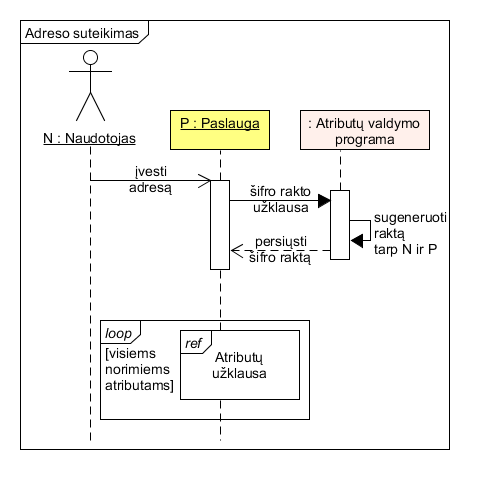
\includegraphics[scale=0.6]{img/userGivesAddress}
    \caption{Naudotojas adreso suteikimas paslaugai}
    \label{fig:userGivesAddress}
\end{figure}

\subsubsection{Paslaugos atliekama atributo užklausa} \label{BCIDM:askForAttribute}

Paslauga P, norinti gauti tam tikrą asmens atributą (pvz. gimimo datą)\footnote{ Paslaugai kreipiantis į kontraktą, ji turi žinoti, koks yra norimo atributo identifikatorius, kurį reikia perduoti į kontrakto funkciją. 
Atributų identifikatoriai gali būti pateikiami atskirame išmaniajame kontrakte arba kuriamo modelio interneto puslapyje.}
, kreipiasi į blokų grandinės išmanųjį kontraktą (žr.\hypertarget{fig:askForAttributeSequence}{~\ref{fig:askForAttributeSequence} pav.}).
Kontraktas tuomet patikrina, ar ši paslauga turi prieigą prie pageidaujamo atributo. Jei turi, tuomet grąžina šį atributą. Jis
užšifruotas paslaugos P turimu šifro raktu, tad paslauga gali jį dešifruoti ir perskaityti duomenis. Jei
naudotojas atmetęs prieigą, apie tai pranešama paslaugai. Jei naudotojas dar nesvarstęs šios prieigos, išsaugoma laukianti
(angl. \textit{pending}) paslaugos P atributo A užklausa ir laukiama naudotojo sprendimo. Naudotojas šią laukiančią užklausą galės pamatyti savo 
atributų valdymo programoje ir ten atlikti sprendimą.

\begin{figure}[h]
    \centering
    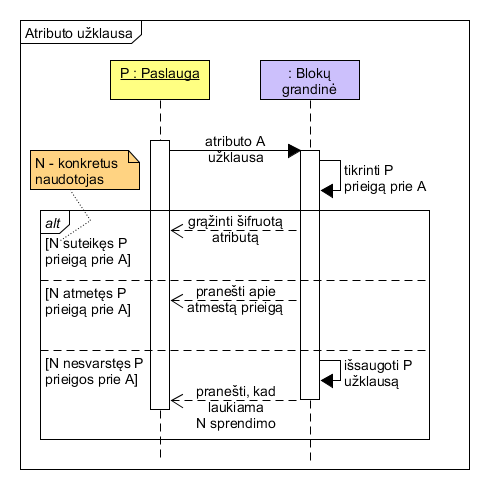
\includegraphics[scale=0.7]{img/askForAttributeSequence}
    \caption{Paslaugos atliekama atributo užklausa}
    \label{fig:askForAttributeSequence}
\end{figure}

\subsubsection{Naudotojo atliekamas paslaugos autorizavimas}

Atributų valdymo programa, stebinti išmaniuosiuose kontraktuose naujas paslaugų užklausas, praneša naudotojui apie dar
neatliktus autorizavimus. Tuomet naudotojas gali pasirinkti, ar suteikti, ar atmesti prieigą prie norimo atributo
A paslaugai P. (žr.\hypertarget{fig:givePermissions}{~\ref{fig:givePermissions} pav.}). Blokų grandinė asmeniui leidžia autorizuoti tik savo naudojamas paslaugas
\footnote{ Ar naudotojo N prieigai pakeisti siunčiamą žinutę tikrai siunčia N, blokų grandinė atskiria iš žinutės parašo.}.

Jei naudotojas prieigą suteikia, tuomet atributų valdymo programa užšifruoja atributą A. Tai
daroma todėl, kad kiekvienas atributas, suteiktas paslaugai P, turi būti užšifruotas tik paslaugai P ir naudotojui N
žinomu šifro raktu bei nusiųstas
į išmanųjį kontraktą. Pati atributo reikšmė yra iš anksto įvesta naudotojo į atributų valdymo programą.
Užšifravus reikšmę, duomenys nusiunčiami į išmanųjį kontraktą ir jame pažymima, kad paslauga P autorizuota
pasiekti atributą A.

Jei naudotojas prieigą atmeta, tuomet blokų grandinėje pažymima, kad paslauga P nėra autorizuota pasiekti atributą A.

Jei naudotojas vėliau nuspręstų pakeisti savo sprendimą (pvz. panaikinti suteiktas prieigas prie atributo A paslaugai P),
jis šį paslaugos autorizavimo procesą galėtų pakartoti ir jau esamai prieigai.


\begin{figure}[h]
    \centering
    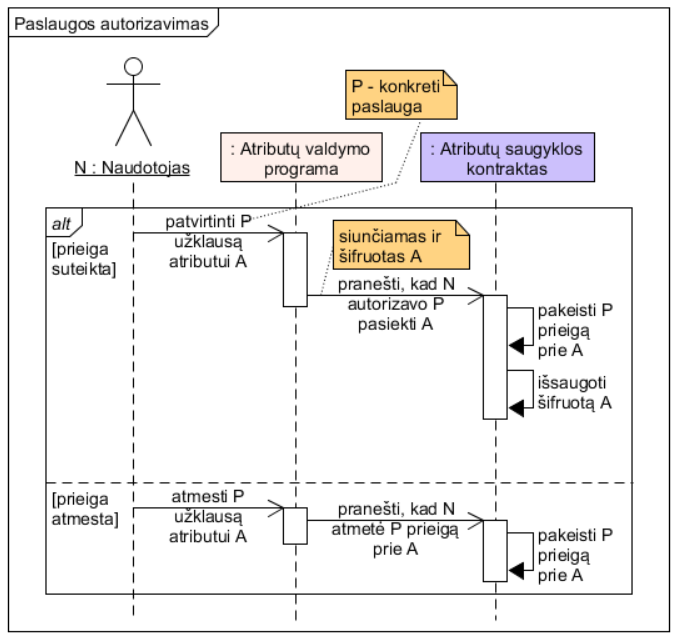
\includegraphics[scale=0.65]{img/givePermissions}
    \caption{Naudotojo atliekamas paslaugos autorizavimas}
    \label{fig:givePermissions}
\end{figure}

\subsubsection{Atributų valdymo programos atliekamas blokų grandinės stebėjimas} \label{BCIDM:blockchainMonitoring}

Blokų grandinės išmanusis kontraktas negali tiesiogiai pranešti išorinei (ne išmaniajame kontrakte esančiai) programai
apie įvykusius pasikeitimus. Todėl išmanusis kontraktas gali saugoti būseną, o ją vėliau pasiekia norinti taikomoji programa.
Tokiu būdu atributų valdymo programa periodiškai kreipiasi į išmanųjį kontraktą ir žiūri, ar yra naujų paslaugų užklausų. Jeigu jų yra,
atributų valdymo programa išsaugo pranešimą apie tai naudotojui (žr.\hypertarget{fig:checkForPendingPermissions}{~\ref{fig:checkForPendingPermissions} pav.}).\\
Panašiu stebėjimo principu pasikeitimus išmaniojo kontrakto būsenoje gali stebėti ir paslaugų tiekėjai
(pvz. apie pasikeitusias prieigas).

\begin{figure}[h]
    \centering
    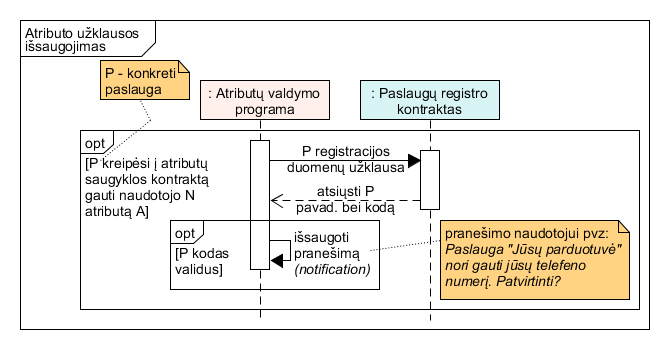
\includegraphics[scale=0.6]{img/checkForPendingPermissions}
    \caption{Atributų valdymo programos atliekamas blokų grandinės stebėjimas}
    \label{fig:checkForPendingPermissions}
\end{figure}